\documentclass{article}
\usepackage[utf8]{inputenc}
\setlength{\parindent}{0em}
\setlength{\parskip}{1.4ex}
\usepackage[danish]{babel}
\usepackage[utf8]{inputenc}
\usepackage{graphicx}
\graphicspath{{pictures/}}
\usepackage{mathtools}
\usepackage{amsfonts,amsmath,amssymb,amsthm} 
\newtheorem{theorem}{Sætning}
\usepackage{cancel}

\title{DM500 Eksamensopgave}

\author{
	Thomas Urup Schjerlund\\
	\texttt{thsch20@student.sdu.dk}
	\and
	Tobias Klink Lehn\\
	\texttt{toleh20@student.sdu.dk}
	\and
	Philip Hayberg Thomsen\\
	\texttt{phtho20@student.sdu.dk}
	\and
	Sean Chrone Græns\\
	\texttt{segra20@student.sdu.dk}
}
\date{15. November 2020}

\begin{document}

\begin{titlepage}
\maketitle
\end{titlepage}

\section{Reeksamen Januar 2012 Opg. 1 - Tobias}
\begin{figure}[h]
\includegraphics[scale=1]{Opgave1Formulering}
\end{figure}

\begin{figure}[h]
\includegraphics[scale=1]{opga}
\end{figure}
\textbf{Svar:}
En afbildning, $\phi: A \rightarrow B$ er bijektiv, hvis og kun hvis funktionen både er \emph{injektiv} (one-to-one) og \emph{surjektiv} (onto).

\begin{theorem}
$f$ er injektiv, hvis $\forall x_1, x_2 \in Dm(f): x_1 \neq x_2 \rightarrow f(x_1) \neq f(x_2)$
\end{theorem}

Sagt på en anden måde, så skal det for alle værdier af x i definitionsmængden gælde, at x hvis to x-værdier er forskellige fra hinanden, så er deres funktionsværdier det også. Helt basalt vil det sige, at to x-værdier ikke kan dele en y-værdi.

Ved at indsætte $x_1$ og $x_2$ og sætte deres funktionsværdi lig hinanden, kan det afgøres hvorvidt det også betyder, at x-værdierne var ens til at starte med - det skal de være, hvis funktionen skal være injektiv:
\begin{center}
\[f(x_1) = x_1^2 + x_1 + 1 \] 
\[ f(x_2)=x_2^2 + x_2 + 1 \] 
\begin{align*}
f(x_1) = f(x_2) \\
\Rightarrow x^2_1 + x_1 + 1 = x^2_2 + x_2 + 1 && \text{Funktionsværdien indsættes} \\
\Leftrightarrow x^2_1 + x_1 = x^2_2 + x_2 && \text{1 går ud på begge sider} \\
\Leftrightarrow x_1^2 = x_2^2 + x_2 - x_1 && \text{$x_1$ trækkes fra på begge sider}\\
\Rightarrow x_1 = \pm\sqrt{x_2^2 + x_2 - x_1} \\
\Rightarrow x_1 = \pm\sqrt{k}  && \text{, $k \in \mathbb{R}$}
\end{align*}
\end{center}

Da det hurtigt viser sig at $x_1 \neq k \Rightarrow f(x_1) = f(k)$, må det betyde, at $x_1$ kan have samme funktionsværdi som et andet tal (forskelligt fra $x_1$) i definitonsmængden ($Dm(f) = \mathbb{R}$), og derfor er \emph{f} ikke injektiv, og derfor automatisk heller ikke bijektiv. For at understrege pointen kan man forsøge sig med $x_1 = 4.91$ og $x_2 = -5.91$ og derfor få:

\begin{align*}
\begin{split}
f(4) = 4.91^2 + 4.91 + 1 \approx 30.02  \\
f(-5.91) = (-5.91)^2 + 5.91 + 1 \approx 30.02
\end{split}
\end{align*}
Af den grund behøver vi ikke kontrollere, om \emph{f} er surjektiv.


\begin{figure}[h]
\includegraphics[scale=1]{opgb}
\end{figure}

\textbf{Svar:} En funktion \emph{f} har en invers, hvis og kun hvis f er bijektiv. Da vi tidligere har konkluderet at \emph{f} ikke er bijektiv, må det også være tilfældet, at \emph{f} ikke er invertibel og derfor ikke har nogen invers.

\begin{figure}[h]
\includegraphics[scale=1]{opgc}
\end{figure}
\textbf{Svar:} To funktioner kan adderes ved at addere deres funktionsforskrifter ved brug af standard algebraiske regler
\begin{align*}
(f+g)(x) = f(x) + g(x) \\
\Rightarrow (f+g)(x) = (x^2 + x + 1) + (2x - 2) && \text{f og g indsættes på deres pladser} \\
= x^2 + x + 1 + 2x - 2 && \text{Ophævning af + parentes} \\
= x^2 + 3x - 1 \\
\end{align*}

\begin{figure}[h]
\includegraphics[scale=1]{opgd}
\end{figure}
\textbf{Svar:} Den sammensatte funktion $f \circ g$ beregnes på følgende vis:
\par
\begin{center}
\begin{math}
f \circ g = f(g(x))
\end{math}
\end{center}

Indsætter man $f$ i $g$ fås:
\begin{center}
\begin{align*}
g(f(x)) = g(x^2 + x + 1) \\
= 2 \cdot (x^2 + x + 1) - 2 && \text{udtrykket indsættes i g} \\
= 2x^2 + 2x + 2 - 2 && \text{Parentesen udregnes} \\
= 2x^2 + 2x
\end{align*}
\end{center}

Dette var løsningen til Opgave 1 i DM527 Reeksamen, Januar 2012.

\section{Reeksamen Februar 2015 Opg. 1 - Thomas}
\begin{figure}[h]
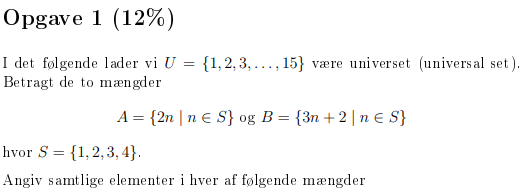
\includegraphics[scale=0.85]{2015Opgave1Formulering}
\end{figure}

\subsection*{Opgave a og b}
Vi starter med at betragte de 2 mængder \emph{A} og \emph{B}.

\begin{center}

$A = \{ 2n | n \in S \}$ \qquad $B = \{ 3n +2 | n \in S \}$

$A = 2 * 1 = 2,$ \qquad $B = 3 * 1 + 2 = 5, $\\
$A = 2 * 2 = 4,$ \qquad $B = 3 * 2 + 2 = 8, $\\
$A = 2 * 3 = 6,$ \qquad $B = 3 * 3 + 2 = 11, $\\
$A = 2 * 4 = 8,$ \qquad $B = 3 * 4 + 2 = 14, $

derfor er

$A = \{ 2, 4, 6, 8 \}$ \qquad $B = \{ 5, 8, 11, 14 \}$
\end{center}

\subsection*{Opgave c}
Angiv samtlige element for $A \cap B$

Fællesmængden er de elementer, som $A$ og $B$ har til fælles:

Så derfor er

\begin{center}
$A \cap B = \{ 8 \}$  
\end{center}

\subsection*{Opgave d}
Angiv samtlige element for $A \cup B$

Foreningsmængden er de elementer, som både findes i $A$ og $B$:

Så derfor er

\begin{center}
$A \cup B = \{ 2, 4, 5, 6, 8, 11, 14 \}$  
\end{center}

\subsection*{Opgave e}
Angiv samtlige element for $A - B$

$A$ fraregnet $B$ betyder de elementer, som findes i mængden A minus de elementer, som er i B:

Så derfor er

\begin{center}
$A - B = \{ 2, 4, 6 \}$  
\end{center}

\subsection*{Opgave f}
Angiv samtlige element for $\bar{A}$

Komplementet af $\bar{A}$ er alle de elementer, som findes i universet, undtagen dem som findes i A:

Så derfor er

\begin{center}
$\bar{A} = \{ 1, 3, 5, 7, 9, 10, 11, 12, 13, 14, 15 \}$  
\end{center}

\section{Philip}
Opgaven tager udgangspunkt i opgave 3 fra eksamensæt 2009, samt en ekstra opgave (gengivet som opgave c i det nedenstående).
Eksamen januar 2009, opgave 3. Opskriv desuden matricen, der repræsenterer relationen R, dog hvor S reduceret til $S = \{1,2,...,6\}$

Lad $S = \{1,2,...,15\}$


a) Hvilke af nedenstående par tilhører R? Hvilke tilhører $R^2$?

\begin{center}
     (1,1) , (2,4) , (4,2) , (3,5) , (2,8)
\end{center}

Vi skal her finde ud af, hvilke par som indeholdeles i R, hvor R er givet, som $R = \{ (a,b)  |  b = 2a\}$.
For at finde ud af hvilke par, som indeholdes i R opstiller vi relationerne for (a,b) og ser, hvorvidt disse par indgår i S for $R = \{ (a,b)  |  b = 2a\}$.


\begin{figure}[h]
\begin{center}
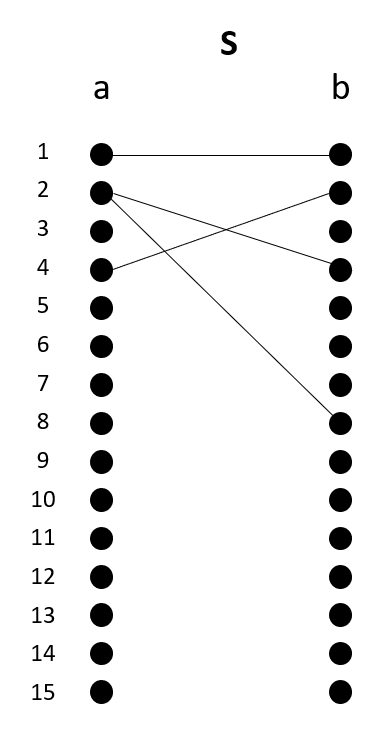
\includegraphics[scale=0.9]{ABC1}
\end{center}
\end{figure}

Af ovenstående figur ses det, at (2,4) er det eneste, som indgår i S. 

Vi ser nu på, hvilke par som indgår i $R^2$.\\
$R^2$ betegner det forhold, at 

\begin{center}
    
    $R^1 = R$ og $R^{n+1} = R^n \circ\ R$
    
\end{center}

Vi finder derfor, at (2,8) indgår i $R^2$, som det eneste par.


b) Opskriv all par i den transitative lukning af R.
Vi skal i denne opgave finde den transitative lukning for ovenstående par. Den transitative lukning kan betegnes som en form for "genvej" mellem relationer således, jf. også nedenstående figur.


\begin{figure}[!h]
\begin{center}
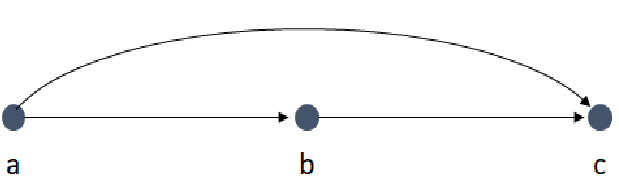
\includegraphics[scale=0.5]{ABC}
\end{center}
\end{figure}

Dette kan vi også skrive, som:

\begin{center}
    $a \geq b$ , $ b \geq c $ og derfor gælder der, at $ a \geq c$
\end{center}

Vi skal derfor finde de par, som gør at ovenstående forhold om transitivitet gælder. Vi finder derfor, at:

\begin{center}
     (1,1) , (2,2) , (2,4) , (2,8) , (3,5) , (4,2) , (4,4)  , (4,8)
\end{center} 

c) Opskriv matricen, der repræsenterer relationen R, dog hvor S reduceret til $S = \{1,2,...,6\}$

R udgør en binær-relation, og vi opskriver derfor matricen, som viser forholdet for $R = \{ (a,b)  |  b = 2a\}$ i 6x6-matricen.

\begin{center}
\begin{math}
R_M = \begin{bmatrix}
0 & 0 & 0 & 0 & 0 & 0\\
1 & 0 & 0 & 0 & 0 & 0\\
0 & 0 & 0 & 0 & 0 & 0\\
0 & 1 & 0 & 0 & 0 & 0\\
0 & 0 & 0 & 0 & 0 & 0\\
0 & 0 & 1 & 0 & 0 & 0\\

\end{bmatrix}
\end{math}
\end{center}









\section{Reeksamen Februar 2015 Opg 3 - Sean}
\section{Opgave 3}
Lad R, S og T være binære relationer på mængden {1, 2, 3, 4}.


% Assignments
\subsection{Opgave A}
Lad \[R = \{(1, 1),(2, 1),(2, 2),(2, 4),(3, 1),(3, 3),(3, 4),(4, 1),(4, 4)\}\]

Er R en partiel ordning?

\textbf{Svar:}
{En partiel ordning er en \emph{relation}, $R$, på en mængde,  hvor $R$ er refleksiv, anti-symmetrisk og transitiv. Det bedømmes hvorvidt $R$ besidder disse egenskaber:}


\subsubsection{Refleksivitet:}
Da sætningen \[\forall a \in A : (a,a) \in R\] betyder at en refleksiv ordning skal relatere enhver værdi til sig selv og da denne er opfyldt kan første krav til en partiel ordning krydses af.


\subsubsection{Antisymmetri:}
Hvis en ordning skal være antisymmetrisk gælder at:\par
\begin{center}
\begin{math}
\forall a,b \in A \land a \neq b: aRb \Rightarrow a  $\bcancel{R}$ b
\end{math}
\end{center}


Her forstås at  Hvis a er relateret til b kan b ikke være relateret til a, medmindre a = b
En anden måde at se om en mængde er antisymmetrisk er ved hjælp af en matrice.\\
\textbf{Matrice for R:}\\ 


\[R=\begin{bmatrix}
1 & 0 & 0 & 0\\
1 & 1 & 0 & 0\\
1 & 0 & 1 & 1\\
1 & 0 & 0 & 1
\end{bmatrix}\]


Sammenligner man værdierne diagonalt og man har en forskellig værdi. Gælder dog ikke to ens 0-værdier, da de i så fald ikke er relateret til hinanden på nogen vis, er relationen antisymmetrisk. 

Her kan man se at R altså er antisymmetrisk.

\subsubsection{Transitivitet}
Her gælder at \[(a,b)\in R \wedge (b,c)\in R \Rightarrow (a,c)\in R, \;  \forall a,b,c \in A\]
Her har vi en binær relation med mængden 1, 2, 3, 4 hvilken betyder at hvis relationen skal være transitiv, skal alle mægnde værdier være i relation med hinanden.
Den transitive lukning ser således ud for relationen \[t(R) = \{(1,1), (2,1), (2,2), (2,4), (3,1), (3,3), (3,4), (4,1), (4,4)\} \cup \{(2,3)\}\]
Her kan vi se relationen forenet med en ny relation, nemlig (2,3), er den transitive lukning af $R$. Af den grund var $R$ ikke transitiv til at starte med, da elementet (2,3) manglede. Da denne ikke er en del a relationen R kan den ikke kaldes transitiv, og dermed er den ikke en partiel ordning.

\vspace{0.5cm}


\subsection{Opgave B}
Lad \[S = \{(1, 2),(2, 3),(2, 4),(4, 2)\}\]


Angiv den transitive lukning af S?
\\\textbf{Svar:}


Som tidligere forklaret er den transitive lukning, samlingen af relationer som der kræves for at relatere enhver værdi med enhver anden. Altså \[(a,b)\in R \wedge (b,c)\in R \Rightarrow (a,c)\in R, \;  \forall a,b,c \in A\]

Altså er lukningen også beksrevet som \[S^*=\bigcup_{i=1}^{\infty} S^i\]

Er der en vej fra den oprindelige relation, kommer der en direkte vej i lukningen.

Har $T$ $n$ elementer kan man skrive \[S^*=\bigcup_{i=1}^{|A|} S^4 = t(S)= \{(1, 2),(2, 3),(2, 4),(4, 2)\}. \cup \{(1,3), (1,4),\} \cup \{(3,4)\}\]



\textbf{Matrice for S:}\\

\[S=\begin{bmatrix}
0 & 1 & 0 & 0\\
0 & 0 & 1 & 1\\
0 & 0 & 0 & 0\\
0 & 1 & 0 & 0
\end{bmatrix}\\\]



\subsection{Opgave C}

Lad \[T = {(1, 1),(1, 3),(2, 2),(2, 4),(3, 1),(3, 3),(4, 2),(4, 4)}\]

Bemærk, at T er en ækvivalens-relation.
Angiv T's ækvivalens-klasser.

Ækvivalens relationer er relationer der er både symmetriske, transitive og refleksive. 

\textbf{Ækvivalens-klasserne for T som følger \[[a] = \{b \vert (a,b) \in R\}\\\]}

\[[1]=\{1,3\}\]
\[[2]=\{2,4\}\\\]

og da \[[1]=[3], [2]=[4]\] fordi \[a\subseteq b\] \[c \in [a] \Rightarrow aRc \Rightarrow bRc \Rightarrow c\in [b]\]
indgår disse i samme klasse.\\

\textbf{Matrice T:}\\

\[T=\begin{bmatrix}
1 & 0 & 1 & 0\\
0 & 1 & 0 & 1\\
1 & 0 & 1 & 0\\
0 & 1 & 1 & 0
\end{bmatrix}\\\]
\pagebreak
\section{Eksamen Februar 2015 Opg. 3 - Alle}
\begin{figure}[h]
\begin{center}
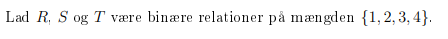
\includegraphics[scale=0.9]{2015Opgave3FormuleringOver}
\end{center}
\end{figure}


\subsection{Underopgave a)}
\begin{figure}[h]
\begin{center}
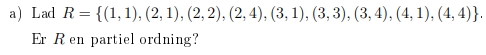
\includegraphics[scale=0.9]{2015Opgave3FormuleringA}
\end{center}
\end{figure}

Hvis en relation, $R$, skal være en partiel ordning, skal relationen være \emph{refleksiv, anti-symmetrisk} og \emph{transitiv}. Mangler den blot én af disse egenskaber, kan relationen ikke være en partiel ordning. Først kontrolleres den refleksive egenskab.

\begin{theorem}
En relation, $R$, på mængden A er refleksiv hvis $\forall a \in A : (a,a) \in R$
\end{theorem}

Fordi $R$ er en relation på mængden $\{1, 2, 3, 4\}$ kræves det, at elementerne (1,1), (2,2), (3,3) og (4,4) er indeholdt i $R$. Dette er tilfældet, og $R$ er derfor refleksiv. Næste egenskab er den anti-symmetriske egenskab.

\begin{theorem}
En relation, $R$, på mængden A er anti-symmetrisk hvis $\forall a,b \in A : (a,b) \in R \Rightarrow (b,a) \notin R \lor a = b$
\end{theorem}

Vi ser allerede at de refleksive elementer findes i $R$. Derudover ses:

\begin{itemize}
\item (2,1) men ikke (1,2)
\item (2,4) men ikke (4,2)
\item (3,1) men ikke (1,3)
\item (3,4) men ikke (4,3)
\item (4,1) men ikke (1,4)
\end{itemize}

Af den grund er $R$ også anti-symmetrisk. Derfor kontrolleres den transitive egenskab som den sidste:

\begin{theorem}
En relation, $R$, på mængden A er transitiv hvis $\forall a,b,c \in A : (a,b)\in R \land (b,c)\in R \Rightarrow (a,c) \in R$
\end{theorem}

Eksempelvis skal (2,1) også findes i $R$ hvis (2,4) og (4,1) eksisterer i R, hvilket også er tilfældet. Elementerne gennemgås slavisk:

\begin{itemize}
\item Da (1,1) er det eneste element med tallet 1 som første element i et par, er der ikke nogen transitivitet at gennemskue. Af den grund kan vi også se bort fra alle elementer i R, hvor 1 indgår. Generelt undgår vi at undersøge mulige transitive elementer ved refleksive elementer, da de altid giver det element, de bliver sammenlignet med i sidste ende.
\item (2,4) og (4,1) medfører $(2,1) \in R$ \checkmark
\item (2,4) og (4,4) medfører $(2,4) \in R$ \checkmark
\item (3,4) og (4,1) medfører $(3,1) \in R$ \checkmark
\end{itemize}

Alle de transitive elementer findes i $R$, og $R$ er derfor også transitiv.

Deraf kan det konkluderes, at $R$ er en partiel ordning.

\subsection{Underopgave b)}

\begin{figure}[h]
\begin{center}
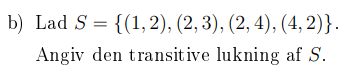
\includegraphics[scale=0.9]{2015Opgave3FormuleringB}
\end{center}
\end{figure}

Den transitive lukning af en relation $R$, er givet ved:

\begin{center}
\begin{math}
R^* = \bigcup_{i = 1}^\infty R^i
\end{math}
\end{center}

hvor $R^i$ er den \emph{i}'te potens af $R$ således at:

\begin{center}
$R^1 = R$
\end{center}
\begin{center}
$R^{i+1} = R \circ R^i$
\end{center}

Omvendt kan det siges, at $R^i$ indeholder de elementer, (a,b), hvor man kan gå på en sti af længe \emph{i} fra a til b i en orienteret graf for relationen. Først findes $S^2$, og derefter arbejdes mod $S^3$ indtil der ikke opstår nye elementer i den sammensatte relation. Når man sammensætter to relationer, $S$ og $R$, vil $S \circ R$ indeholde de elementer, (a,c), der opstår, når man går fra (a,b) i $R$ til (b,c) i $S$.

\begin{center}
\begin{math}
S^2 = S \circ S = \{(1,3), (1,4), (2,2), (4,4)\}
\end{math}
\par
\begin{math}
S^3 = S \circ S^2 = \{(1,2), (2,3), (2,4), (4,2))\}
\end{math}
\end{center}
\par 
Det ses her at $S^3 = S$, og der dannes derfor ikke flere par. Derfor er den transitive lukning af S:

\begin{center}
\begin{math}
S^* = S \cup S^2 = \{(1,2), (1,3), (1,4), (2,2), (2,3), (2,4), (4,2), (4,4)\}
\end{math}
\end{center}

Følger man samme procedure med at kontrollere de transitive elementer fra opgave a), vil man se, at dette er den transitive lukning.

\subsection{Underopgave c)}
\begin{figure}[h]
\begin{center}
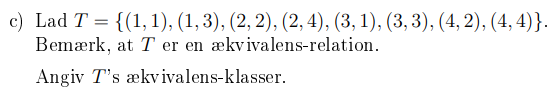
\includegraphics[scale=0.8]{2015Opgave3FormuleringC}
\end{center}
\end{figure}

\begin{theorem}
En ækvivalensklasse, $[a]_R = \{b \in R | aRb\}$
\end{theorem}

Sagt på en anden måde er ækvivalensklassen for et element, \emph{a}, i $R$ alle de elementer, som \emph{a} er relateret til. Vi opskriver derfor:

\begin{center}
$[1]_T = \{1, 3\}$ \par
$[2]_T = \{2, 4\}$ \par 
$[3]_T = [1]_T$ \par
$[4]_T = [2]_T$
\end{center}

På grund af refleksivitet vil et element altid have sig selv i sin ækvivalensklasse, og symmetrien medfører at to elementer altid vil have hinanden i sine ækvivalensklasser, hvis de er relateret til hinanden. Grundet transitiviteten vil to elementer altid være i hinandens ækvivalensklasse, hvis et tredje element er relateret til dem begge.
Det ses desuden at ækvivalænsklasserne udgør en partitionering af mængden $C$, som T er en relationen på.

\subsection{Underopgave fra Take-Home-Eksamen}
\begin{center}
Opskriv desuden matricerne, der repræsenterer de tre relationer \emph{R, S} og \emph{T}.
\end{center}

$R$, $S$ og $T$ er alle binære relationer. Hver række, \emph{i}, i matricen, M, beskriver et element, a, og hvis der står et 1-tal på plads $M_i,j$, betyder det, at \emph{a} er relateret til \emph{b}, som er beskrevet i kolonnen \emph{j}. Ellers står der et 0.

\begin{center}
\begin{math}
R_M = \begin{bmatrix}
1 & 0 & 0 & 0 \\
1 & 1 & 0 & 1 \\
1 & 0 & 1 & 1 \\
1 & 0 & 0 & 1 
\end{bmatrix} 
\end{math}\par 
\begin{math}
S_M = \begin{bmatrix}
0 & 1 & 0 & 0 \\
0 & 0 & 1 & 1 \\
0 & 0 & 0 & 0 \\
0 & 1 & 0 & 0 
\end{bmatrix}
\end{math} \par 
\begin{math}
T_M = \begin{bmatrix}
1 & 0 & 1 & 0 \\
0 & 1 & 0 & 1 \\
1 & 0 & 1 & 0 \\
0 & 1 & 0 & 1 \\
\end{bmatrix}
\end{math}
\end{center}

\end{document}
